\documentclass[tikz,border=5mm]{standalone}
\usepackage{helvet}
\renewcommand{\familydefault}{\sfdefault}
\usetikzlibrary{positioning, arrows.meta, shapes.geometric, backgrounds, fit, calc}
\usepackage{xcolor}

\definecolor{boxblue}{RGB}{225, 240, 255}
\definecolor{boxgreen}{RGB}{235, 250, 225}
\definecolor{boxpurple}{RGB}{240, 235, 255}
\definecolor{orangelink}{RGB}{255, 120, 0}
\definecolor{greenlink}{RGB}{0, 160, 100}

\begin{document}
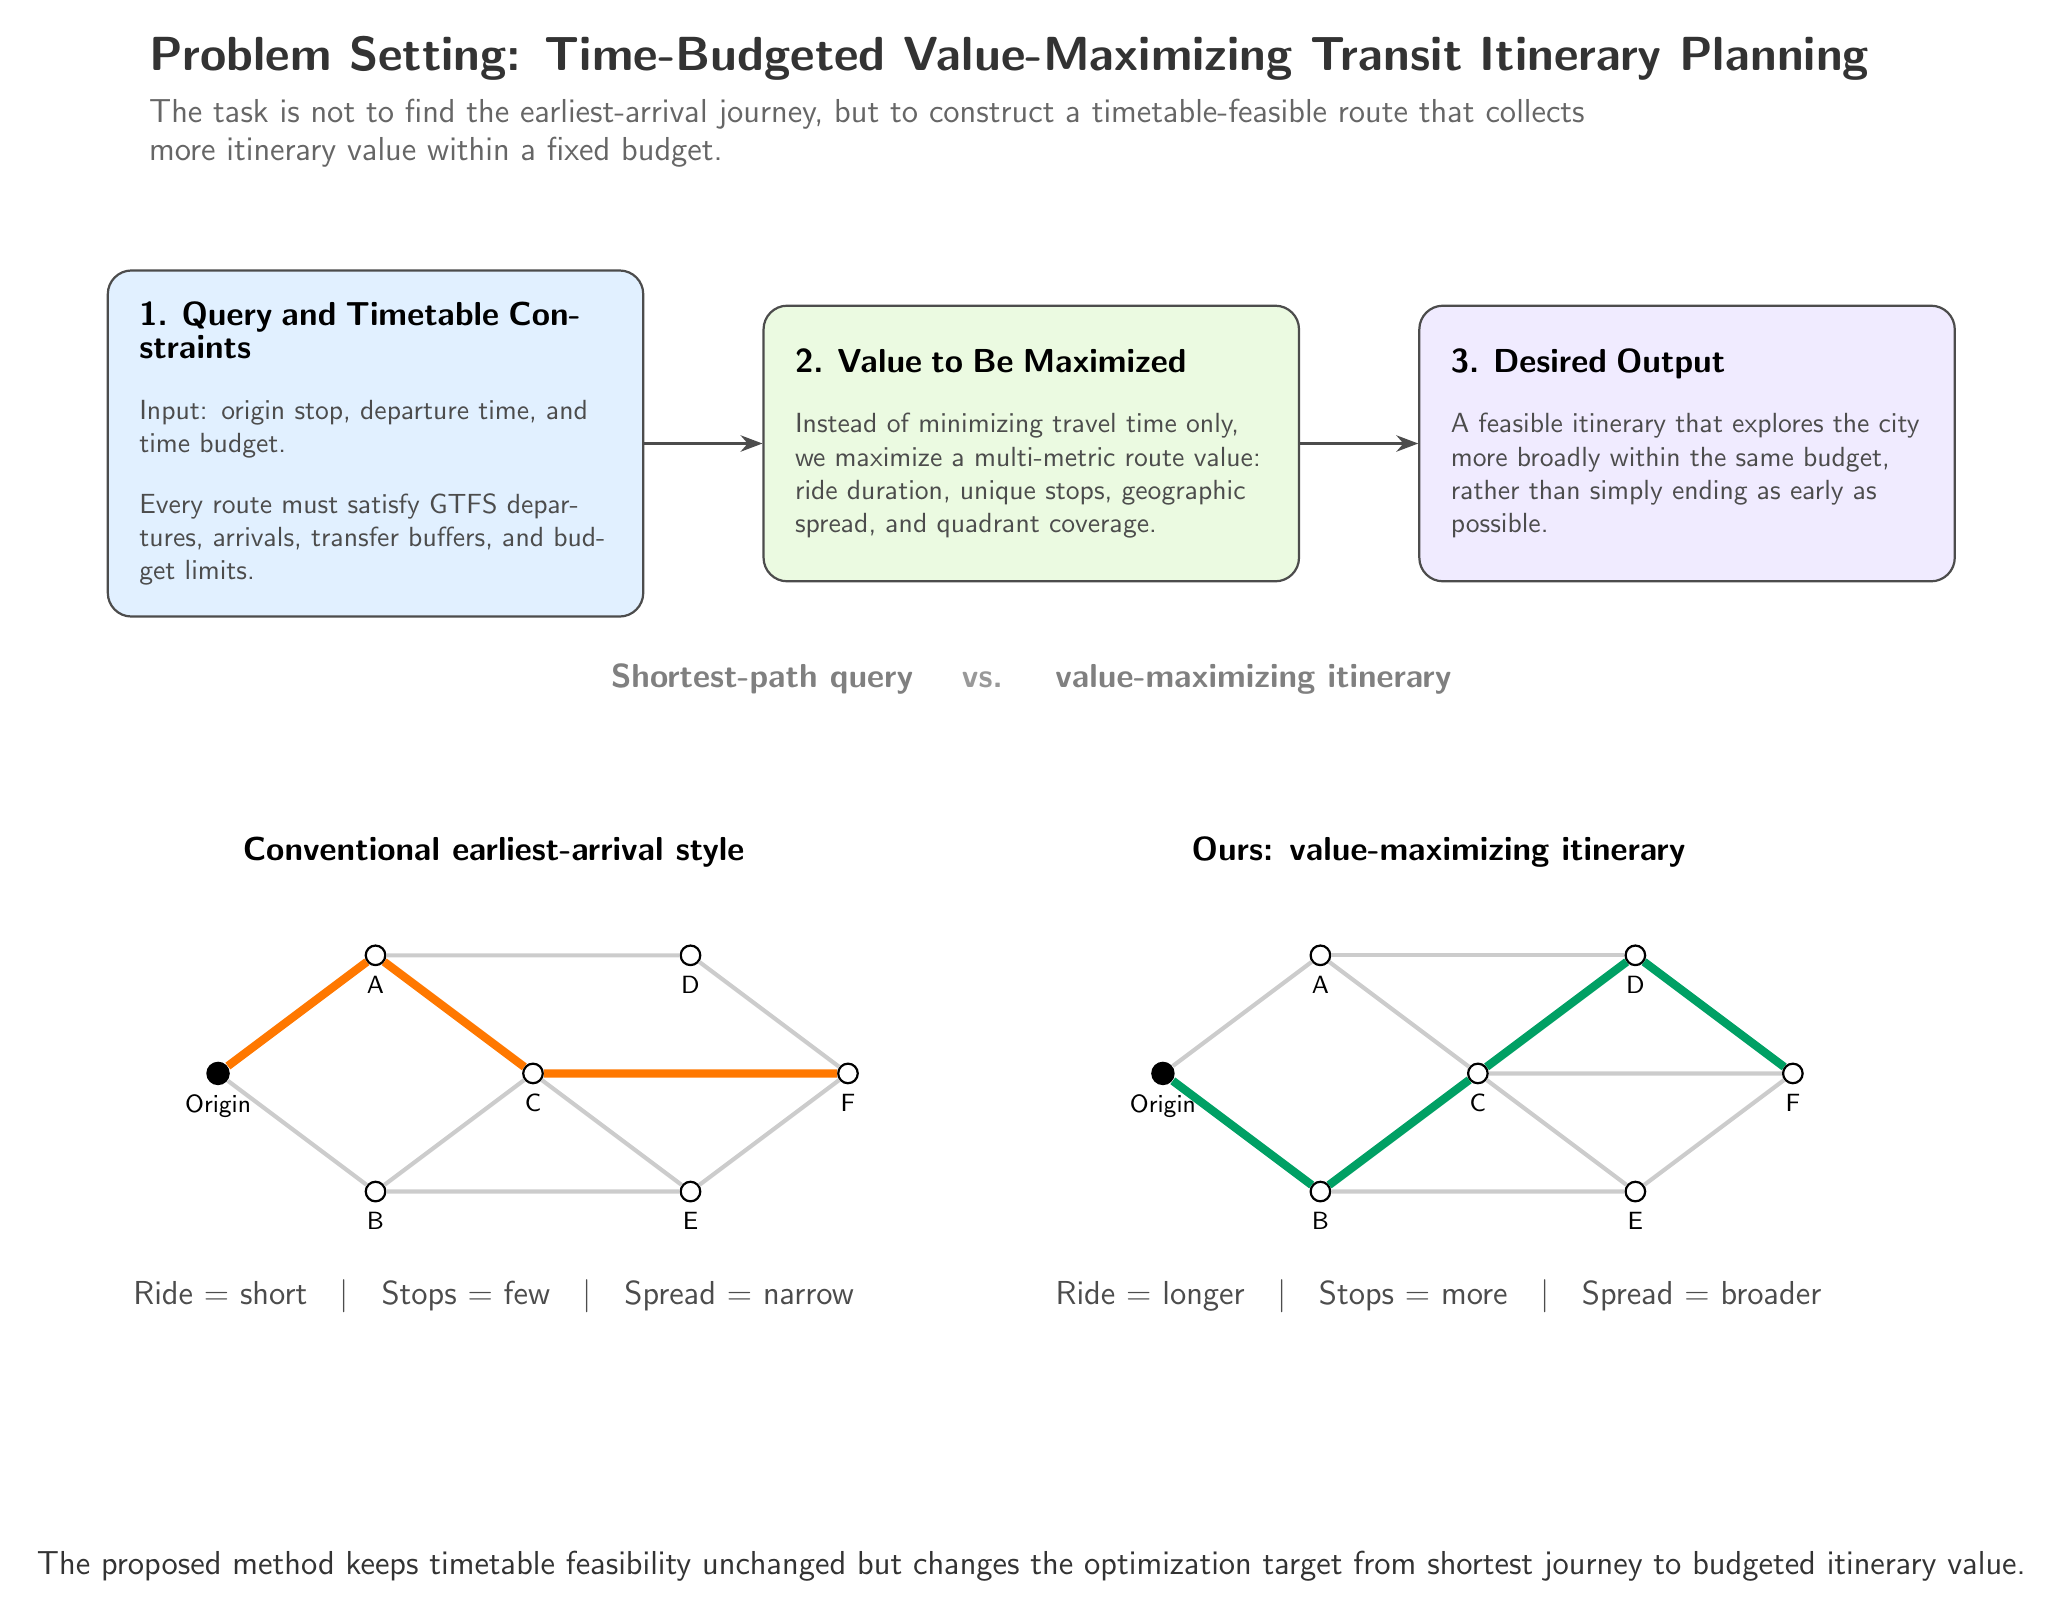
\begin{tikzpicture}[
    box/.style={draw=black!70, thick, rounded corners=3mm, fill=#1, text width=6cm, minimum height=3.5cm, align=left, inner sep=4mm},
    arrow/.style={-{Stealth[scale=1.2]}, thick, draw=black!70},
    gedge/.style={draw=black!20, line width=1.5pt},
    oedge/.style={draw=orangelink, line width=3pt},
    greenedge/.style={draw=greenlink, line width=3pt},
    node distance=1.5cm,
    font=\sffamily
]

% Title
\node[anchor=south west, font=\LARGE\bfseries, text=black!80] (title) at (0, 4.5) {Problem Setting: Time-Budgeted Value-Maximizing Transit Itinerary Planning};
\node[anchor=north west, font=\large, text=black!60, text width=19cm] (subtitle) at (title.south west) {The task is not to find the earliest-arrival journey, but to construct a timetable-feasible route that collects more itinerary value within a fixed budget.};

% Top 3 Boxes
\node[box=boxblue] (box1) at (3, 0) {
    \textbf{\large 1. Query and Timetable Constraints}\\[10pt]
    \textcolor{black!70}{Input: origin stop, departure time, and time budget.}\\[10pt]
    \textcolor{black!70}{Every route must satisfy GTFS departures, arrivals, transfer buffers, and budget limits.}
};

\node[box=boxgreen, right=of box1] (box2) {
    \textbf{\large 2. Value to Be Maximized}\\[10pt]
    \textcolor{black!70}{Instead of minimizing travel time only, we maximize a multi-metric route value: ride duration, unique stops, geographic spread, and quadrant coverage.}
};

\node[box=boxpurple, right=of box2] (box3) {
    \textbf{\large 3. Desired Output}\\[10pt]
    \textcolor{black!70}{A feasible itinerary that explores the city more broadly within the same budget, rather than simply ending as early as possible.}
};

\draw[arrow] (box1) -- (box2);
\draw[arrow] (box2) -- (box3);

% Transition arrows or text
\node[align=center, font=\large\bfseries, text=black!50] at ($ (box1.south)!0.5!(box3.south) + (0, -1cm) $) {Shortest-path query \quad \textcolor{black!40}{vs.} \quad value-maximizing itinerary};

% Bottom Graphs
% Left: Conventional earliest-arrival
\begin{scope}[yshift=-8cm, xshift=1cm]
    \node[font=\large\bfseries, anchor=south, align=center] at (3.5, 2.5) {Conventional earliest-arrival style};
    
    % Nodes
    \node[circle, fill=black, inner sep=3pt, label={[font=\small]below:Origin}] (o1) at (0, 0) {};
    \node[circle, draw=black, thick, fill=white, inner sep=2.5pt, label={[font=\small]below:A}] (a1) at (2, 1.5) {};
    \node[circle, draw=black, thick, fill=white, inner sep=2.5pt, label={[font=\small]below:B}] (b1) at (2, -1.5) {};
    \node[circle, draw=black, thick, fill=white, inner sep=2.5pt, label={[font=\small]below:C}] (c1) at (4, 0) {};
    \node[circle, draw=black, thick, fill=white, inner sep=2.5pt, label={[font=\small]below:D}] (d1) at (6, 1.5) {};
    \node[circle, draw=black, thick, fill=white, inner sep=2.5pt, label={[font=\small]below:E}] (e1) at (6, -1.5) {};
    \node[circle, draw=black, thick, fill=white, inner sep=2.5pt, label={[font=\small]below:F}] (f1) at (8, 0) {};
    
    % Gray Edges
    \draw[gedge] (o1) -- (b1) -- (c1);
    \draw[gedge] (b1) -- (e1) -- (f1);
    \draw[gedge] (a1) -- (d1) -- (f1);
    \draw[gedge] (c1) -- (e1);
    
    % Orange Edges (shortest path)
    \draw[oedge] (o1) -- (a1) -- (c1) -- (f1);
    
    \node[font=\large, text=black!70, anchor=north] at (3.5, -2.5) {Ride = short \ \ $\mid$ \ \ Stops = few \ \ $\mid$ \ \ Spread = narrow};
\end{scope}

% Right: Ours: value-maximizing
\begin{scope}[yshift=-8cm, xshift=13cm]
    \node[font=\large\bfseries, anchor=south, align=center] at (3.5, 2.5) {Ours: value-maximizing itinerary};
    
    % Nodes (re-drawn)
    \node[circle, fill=black, inner sep=3pt, label={[font=\small]below:Origin}] (o2) at (0, 0) {};
    \node[circle, draw=black, thick, fill=white, inner sep=2.5pt, label={[font=\small]below:A}] (a2) at (2, 1.5) {};
    \node[circle, draw=black, thick, fill=white, inner sep=2.5pt, label={[font=\small]below:B}] (b2) at (2, -1.5) {};
    \node[circle, draw=black, thick, fill=white, inner sep=2.5pt, label={[font=\small]below:C}] (c2) at (4, 0) {};
    \node[circle, draw=black, thick, fill=white, inner sep=2.5pt, label={[font=\small]below:D}] (d2) at (6, 1.5) {};
    \node[circle, draw=black, thick, fill=white, inner sep=2.5pt, label={[font=\small]below:E}] (e2) at (6, -1.5) {};
    \node[circle, draw=black, thick, fill=white, inner sep=2.5pt, label={[font=\small]below:F}] (f2) at (8, 0) {};
    
    % Gray Edges
    \draw[gedge] (o2) -- (a2) -- (c2) -- (f2);
    \draw[gedge] (a2) -- (d2);
    \draw[gedge] (b2) -- (e2) -- (f2);
    \draw[gedge] (c2) -- (e2);
    
    % Green Edges (value maximizing)
    \draw[greenedge] (o2) -- (b2) -- (c2) -- (d2) -- (f2);
    
    \node[font=\large, text=black!70, anchor=north] at (3.5, -2.5) {Ride = longer \ \ $\mid$ \ \ Stops = more \ \ $\mid$ \ \ Spread = broader};
\end{scope}

% Bottom Text
\node[align=center, font=\large, text=black!80, anchor=south] at ($ (box2.south) + (0, -12.8cm) $) {The proposed method keeps timetable feasibility unchanged but changes the optimization target from shortest journey to budgeted itinerary value.};

\end{tikzpicture}
\end{document}
